\section{Analysis}\label{sec:analysis}

\subsection{The data samples}
The datasamples used for the analysis have been preselected with either an electron or muontrigger. In the preselection a lepton and jet transverse momentum 
$\texttt{lep\_pt}, \, \texttt{jet\_pt} > 25 \, \si{\giga\eV}$ and a pseudorapidity for jets and lepton of $|\eta| <2.5$. 
The samples are saved in \texttt{ntuples}. Sometimes an entry for a variable contains more entries than the \texttt{ntuple} itself since if a multiple 
electrons or jets are measured for every lepton or jet a new entry is created. An example for such a variable is the lepton transverse momentum 
shown in Figure \ref{fig:unselected_pt} with 467238 entries while the data sample has 450199 entries.  
Furthermore the figure contains the mean value and the standard deviation of the variable. The unit of the transverse momentum in the data is $\si{\mega\eV}$.

\begin{figure}[tb]
    \centering
    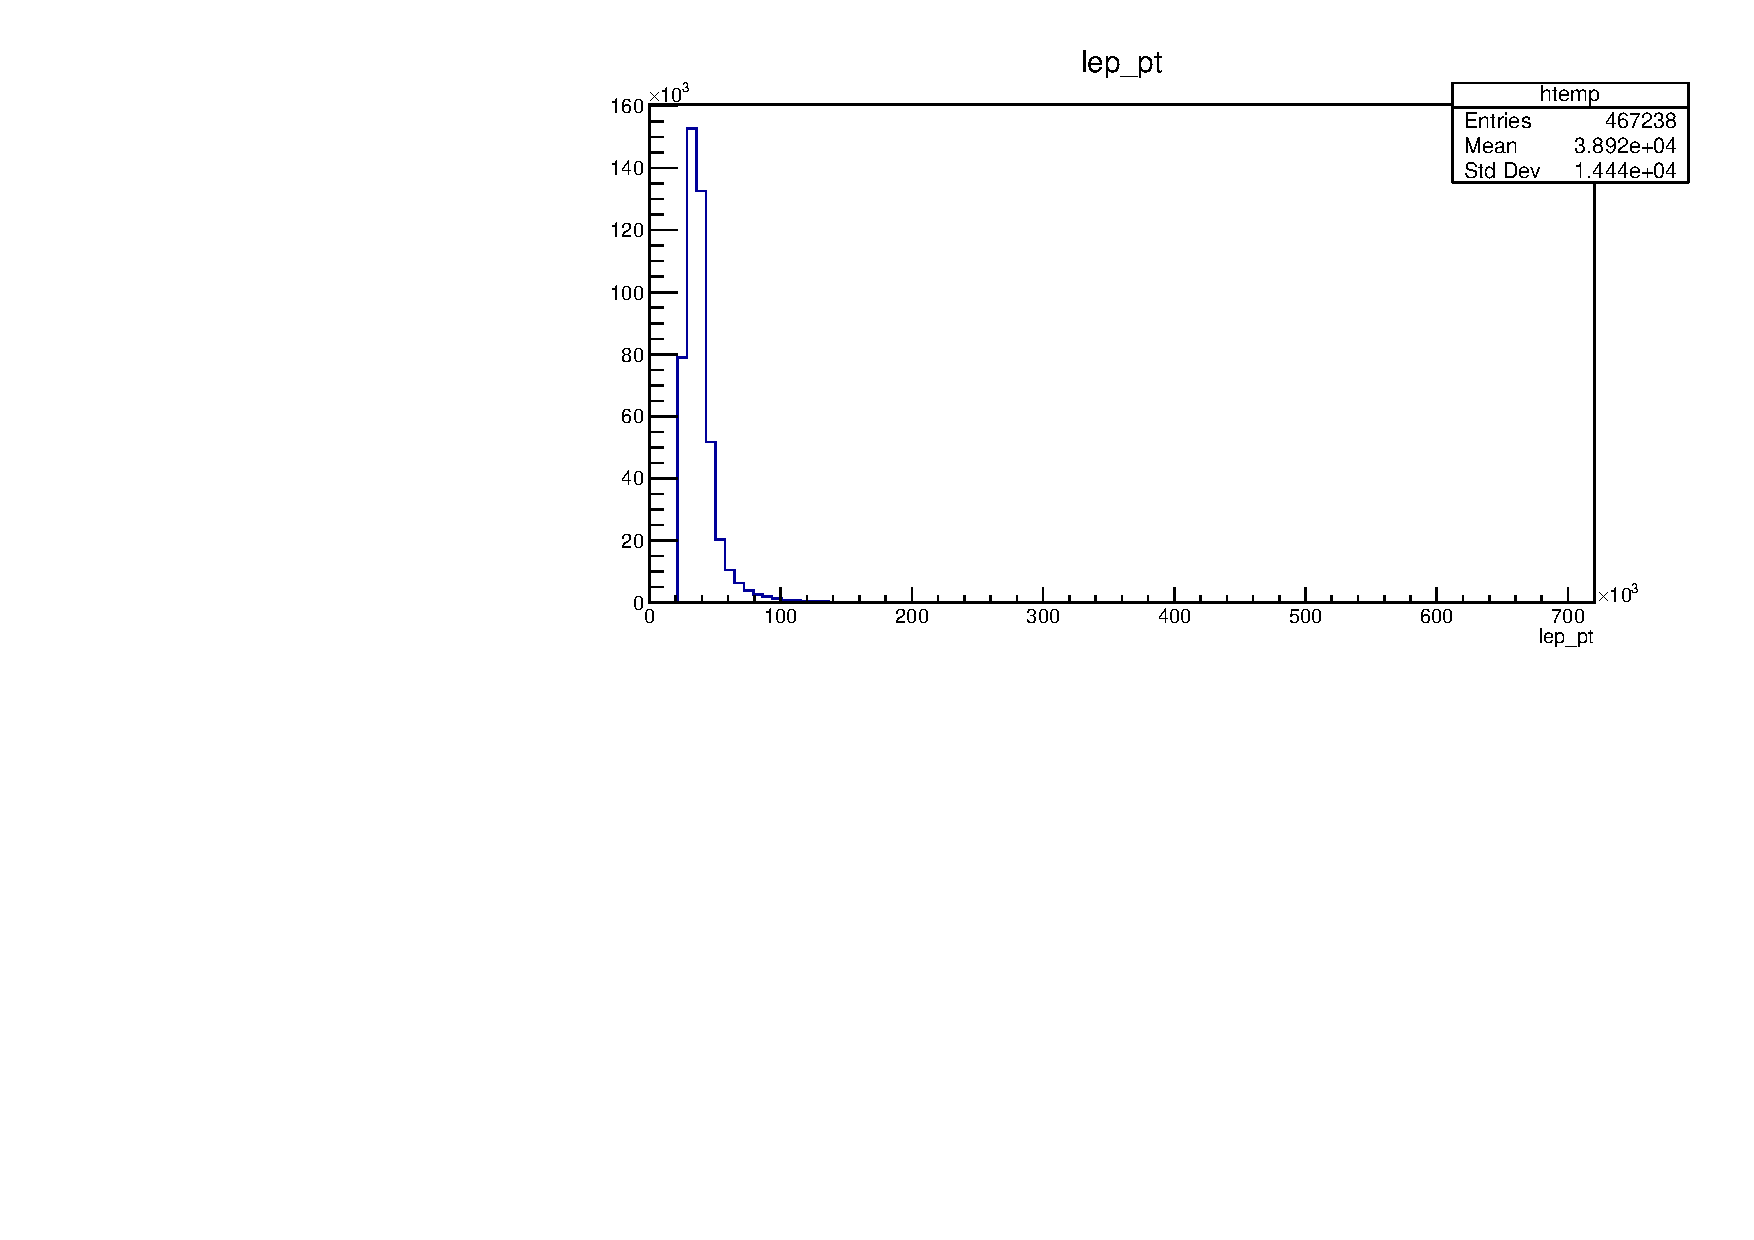
\includegraphics[width=.9\textwidth]{plots/TBrowser_hist.pdf}
    \caption{Histogram of the transverse momentum of the leptons in from one of the data samples created with the \texttt{TBrowser} environment from \texttt{Root}.}
    \label{fig:unselected_pt}
  \end{figure}

\subsection{The event selection}
This analysis focuses on the $\texttt{lepton+jets}$ final state where the final state consists of one charged lepton, a neutrino, two bottom quarks and two other quarks from a 
decay of a W boson. Therefore in the selection requirements are introduced to select for the final state. 
For the jets the number of good jets in one event has to be $\geq 4$ (Cut 1) while exactly one lepton is required (Cut 2) 
in the events. Since the final state contains a neutrino which is not seen in the detector a missing 
transverse energy $met\_et > 40 \, \si{\giga\eV}$ (Cut 3) is required. To supress combinatorial background 
the lepton is required to have a transverse momentum $lep\_pt > 50 \, \si{\giga\eV}$ (Cut 4) and one of 
the jets has to pass $jet\_pt > 80 \, \si{\giga\eV}$ (Cut 5). The number of b-tagged jets in one event has to be 
$\geq 2$ (Cut 6) and one of the b-jets has to fulfill $\texttt{jet\_pt} > 50 \, \si{\giga\eV}$ (Cut 7).
The efficiency of the selection calculated after subsequent application of the cuts is shown in figure 
% original table table with the efficiencies
%\begin{table}[]
%    \begin{tabular}{l|lllllll}
%    sample             & Cut 1 & Cut 2 & Cut 3 & Cut 4     & Cut 5  &  Cut 6 & Cut 7 \\
%    \hline
%      %data.el.0     & 0.00531987 & 0.0051666  & 0.00281875 & 0.00138605  & 0.00101955  & 0.000251    & 0.000228788 \\
%      %data.el.1     & 0.00529988 & 0.0051555  & 0.00279876 & 0.00147935  & 0.00111284  & 0.000288761 & 0.00026877  \\
%      %data.el.2     & 0.00512884 & 0.00501112 & 0.00268104 & 0.00126166  & 0.000937363 & 0.000242115 & 0.000224345 \\
%      %data.el.3     & 0.00531321 & 0.0051866  & 0.00292093 & 0.00148379  & 0.00111506  & 0.000299867 & 0.000279876 \\
%      %data.el.4     & 0.00510885 & 0.00498891 & 0.00269214 & 0.00134829  & 0.00100622  & 0.000255443 & 0.000237673 \\
%      %data.el.5     & 0.00526656 & 0.0050933  & 0.00277655 & 0.00138605  & 0.00108174  & 0.000270991 & 0.000248779 \\
%      %data.el.6     & 0.00499113 & 0.00484452 & 0.00258997 & 0.00130831  & 0.00100622  & 0.000246558 & 0.000224345 \\
%      %data.el.7     & 0.00509997 & 0.00498668 & 0.00267882 & 0.00124834  & 0.000926257 & 0.000253221 & 0.000226566 \\
%      %data.el.8     & 0.00519549 & 0.00505333 & 0.00266105 & 0.00128388  & 0.000966242 & 0.000251001 & 0.000244337 \\
%      %data.el.9     & 0.00529545 & 0.00517328 & 0.00290539 & 0.00147491  & 0.0011506   & 0.000308753 & 0.000286541 \\
%      %data.el       & 0.00520192 & 0.00506598 & 0.00275234 & 0.00136606  & 0.00103221  & 0.000266771 & 0.000247002 \\
%      %data.mu.0     & 0.00456057 & 0.00440073 & 0.00265678 & 0.0012538   & 0.000969653 & 0.000241525 & 0.000223766 \\
%      %data.mu.1     & 0.00438298 & 0.00422848 & 0.00254312 & 0.00119875  & 0.000903946 & 0.000202455 & 0.000190024 \\
%      %data.mu.2     & 0.00458544 & 0.00440074 & 0.00272427 & 0.00129465  & 0.000990966 & 0.000232646 & 0.000213111 \\
%      %data.mu.3     & 0.00442738 & 0.00428708 & 0.00266033 & 0.00125558  & 0.000966103 & 0.000268165 & 0.000248629 \\
%      %data.mu.4     & 0.00448243 & 0.00432082 & 0.00260173 & 0.00124137  & 0.000948344 & 0.000225542 & 0.000204231 \\
%      %data.mu.5     & 0.00454104 & 0.00434746 & 0.00261061 & 0.00121828  & 0.000946568 & 0.000243302 & 0.000225542 \\
%      %data.mu.6     & 0.00447355 & 0.00431727 & 0.00272604 & 0.00129465  & 0.0010176   & 0.000257509 & 0.000243302 \\
%      %data.mu.7     & 0.00431194 & 0.00414501 & 0.00252359 & 0.00126268  & 0.000935912 & 0.000243302 & 0.000232646 \\
%      %data.mu.8     & 0.00454814 & 0.00436522 & 0.00269408 & 0.00124847  & 0.000960775 & 0.00027882  & 0.000255733 \\
%      %data.mu.9     & 0.00439896 & 0.00422848 & 0.00258752 & 0.00119342  & 0.000921705 & 0.000252181 & 0.000232646 \\
%      %data.mu       & 0.00447124 & 0.00430413 & 0.00263281 & 0.00124617  & 0.000956158 & 0.000244545 & 0.000226963 \\
%      diboson.el    & 0.0202309  & 0.0194924  & 0.010668   & 0.00565275  & 0.00371891  & 0.000127506 & 0.00011688  \\
%      diboson.mu    & 0.016195   & 0.0149084  & 0.0093971  & 0.00480721  & 0.00313382  & 9.99691e-05 & 9.56227e-05 \\
%      singletop.el  & 0.0906053  & 0.0899371  & 0.0628734  & 0.0336544   & 0.0262382   & 0.00835954  & 0.00795335  \\
%      singletop.mu  & 0.0890013  & 0.0881404  & 0.0624559  & 0.0311724   & 0.0238848   & 0.00794863  & 0.00747094  \\
%      ttbar.el      & 0.436571   & 0.427593   & 0.307784   & 0.163033    & 0.128469    & 0.053868    & 0.0505078   \\
%      ttbar.mu      & 0.434872   & 0.424322   & 0.306789   & 0.154734    & 0.121542    & 0.0513304   & 0.0482129   \\
%      wjets.el      & 0.00489397 & 0.00489397 & 0.00311956 & 0.00159742  & 0.00125348  & 1.66945e-05 & 1.42213e-05 \\
%      wjets.mu      & 0.00482915 & 0.00482903 & 0.00312312 & 0.00150353  & 0.00115609  & 1.74563e-05 & 1.52894e-05 \\
%      zjets.el      & 0.0118665  & 0.0106797  & 0.00297376 & 0.00170699  & 0.00117077  & 5.65506e-05 & 5.25442e-05 \\
%      zjets.mu      & 0.00627221 & 0.0040402  & 0.0015754  & 0.000833442 & 0.00062556  & 3.62866e-05 & 3.3859e-05  \\
%      zprime400.el  & 0.336048   & 0.330579   & 0.222776   & 0.0988089   & 0.0562713   & 0.0238211   & 0.0226057   \\
%      zprime400.mu  & 0.339518   & 0.335549   & 0.230281   & 0.0935609   & 0.0595297   & 0.0242088   & 0.0222244   \\
%      zprime500.el  & 0.418102   & 0.411958   & 0.298848   & 0.16983     & 0.137905    & 0.0554032   & 0.0502468   \\
%      zprime500.mu  & 0.401054   & 0.394935   & 0.28328    & 0.152137    & 0.122952    & 0.0505555   & 0.0480136   \\
%      zprime750.el  & 0.537326   & 0.524537   & 0.427844   & 0.30235     & 0.293616    & 0.125702    & 0.121439    \\
%      zprime750.mu  & 0.532581   & 0.517974   & 0.424298   & 0.292574    & 0.283128    & 0.127263    & 0.124814    \\
%      zprime1000.el & 0.594403   & 0.581055   & 0.503445   & 0.38859     & 0.383423    & 0.180301    & 0.177395    \\
%      zprime1000.mu & 0.609297   & 0.587992   & 0.50066    & 0.377674    & 0.3716      & 0.168941    & 0.166124    \\
%      zprime1250.el & 0.614838   & 0.597018   & 0.530515   & 0.417424    & 0.413231    & 0.191009    & 0.18798     \\
%      zprime1250.mu & 0.630988   & 0.608626   & 0.537332   & 0.420378    & 0.415793    & 0.19302     & 0.190494    \\
%      zprime1500.el & 0.630429   & 0.610937   & 0.557169   & 0.447279    & 0.443878    & 0.190084    & 0.185767    \\
%      zprime1500.mu & 0.639837   & 0.615859   & 0.555766   & 0.445229    & 0.441747    & 0.188737    & 0.18635     \\
%      zprime1750.el & 0.637424   & 0.619702   & 0.566091   & 0.462266    & 0.458721    & 0.191257    & 0.189632    \\
%      zprime1750.mu & 0.642951   & 0.61898    & 0.565701   & 0.452713    & 0.449444    & 0.189475    & 0.187623    \\
%      zprime2000.el & 0.636319   & 0.613722   & 0.563779   & 0.450139    & 0.446209    & 0.174063    & 0.17177     \\
%      zprime2000.mu & 0.659439   & 0.635841   & 0.58541    & 0.468376    & 0.464902    & 0.180283    & 0.179085    \\
%      zprime2250.el & 0.63421    & 0.614402   & 0.567938   & 0.448538    & 0.446316    & 0.168456    & 0.16716     \\
%      zprime2250.mu & 0.652435   & 0.628021   & 0.580443   & 0.471391    & 0.468386    & 0.180669    & 0.178165    \\
%      zprime2500.el & 0.636889   & 0.618791   & 0.56315    & 0.442434    & 0.438776    & 0.1598      & 0.157682    \\
%      zprime2500.mu & 0.658653   & 0.635011   & 0.585602   & 0.471245    & 0.466729    & 0.175721    & 0.172799    \\
%      zprime3000.el & 0.6        & 0.584015   & 0.524453   & 0.394481    & 0.385728    & 0.147288    & 0.145005    \\
%      zprime3000.mu & 0.626332   & 0.604459   & 0.546971   & 0.430875    & 0.424285    & 0.160684    & 0.15816     
%    \end{tabular}
%    \end{table}

%\begin{figure}

  \begin{table}[]
    \begin{tabular}{l|lllllll}
    sample             & Cut 1 & Cut 2 & Cut 3 & Cut 4     & Cut 5   \\
    \hline
      diboson.el    & 0.0202309  & 0.0194924  & 0.010668   & 0.00565275  & 0.00371891  \\
      diboson.mu    & 0.016195   & 0.0149084  & 0.0093971  & 0.00480721  & 0.00313382  \\
      singletop.el  & 0.0906053  & 0.0899371  & 0.0628734  & 0.0336544   & 0.0262382   \\
      singletop.mu  & 0.0890013  & 0.0881404  & 0.0624559  & 0.0311724   & 0.0238848   \\
      ttbar.el      & 0.436571   & 0.427593   & 0.307784   & 0.163033    & 0.128469    \\
      ttbar.mu      & 0.434872   & 0.424322   & 0.306789   & 0.154734    & 0.121542    \\
      wjets.el      & 0.00489397 & 0.00489397 & 0.00311956 & 0.00159742  & 0.00125348  \\
      wjets.mu      & 0.00482915 & 0.00482903 & 0.00312312 & 0.00150353  & 0.00115609  \\
      zjets.el      & 0.0118665  & 0.0106797  & 0.00297376 & 0.00170699  & 0.00117077  \\
      zjets.mu      & 0.00627221 & 0.0040402  & 0.0015754  & 0.000833442 & 0.00062556  \\
      zprime400.el  & 0.336048   & 0.330579   & 0.222776   & 0.0988089   & 0.0562713   \\
      zprime400.mu  & 0.339518   & 0.335549   & 0.230281   & 0.0935609   & 0.0595297   \\
      zprime500.el  & 0.418102   & 0.411958   & 0.298848   & 0.16983     & 0.137905    \\
      zprime500.mu  & 0.401054   & 0.394935   & 0.28328    & 0.152137    & 0.122952    \\
      zprime750.el  & 0.537326   & 0.524537   & 0.427844   & 0.30235     & 0.293616    \\
      zprime750.mu  & 0.532581   & 0.517974   & 0.424298   & 0.292574    & 0.283128    \\
      zprime1000.el & 0.594403   & 0.581055   & 0.503445   & 0.38859     & 0.383423    \\
      zprime1000.mu & 0.609297   & 0.587992   & 0.50066    & 0.377674    & 0.3716      \\
      zprime1250.el & 0.614838   & 0.597018   & 0.530515   & 0.417424    & 0.413231    \\
      zprime1250.mu & 0.630988   & 0.608626   & 0.537332   & 0.420378    & 0.415793    \\
      zprime1500.el & 0.630429   & 0.610937   & 0.557169   & 0.447279    & 0.443878    \\
      zprime1500.mu & 0.639837   & 0.615859   & 0.555766   & 0.445229    & 0.441747    \\
      zprime1750.el & 0.637424   & 0.619702   & 0.566091   & 0.462266    & 0.458721    \\
      zprime1750.mu & 0.642951   & 0.61898    & 0.565701   & 0.452713    & 0.449444    \\
      zprime2000.el & 0.636319   & 0.613722   & 0.563779   & 0.450139    & 0.446209    \\
      zprime2000.mu & 0.659439   & 0.635841   & 0.58541    & 0.468376    & 0.464902    \\
      zprime2250.el & 0.63421    & 0.614402   & 0.567938   & 0.448538    & 0.446316    \\
      zprime2250.mu & 0.652435   & 0.628021   & 0.580443   & 0.471391    & 0.468386    \\
      zprime2500.el & 0.636889   & 0.618791   & 0.56315    & 0.442434    & 0.438776    \\
      zprime2500.mu & 0.658653   & 0.635011   & 0.585602   & 0.471245    & 0.466729    \\
      zprime3000.el & 0.6        & 0.584015   & 0.524453   & 0.394481    & 0.385728    \\
      zprime3000.mu & 0.626332   & 0.604459   & 0.546971   & 0.430875    & 0.424285    
    \end{tabular}
    %\end{table}
    \caption{The efficiency of the selection after the application of subsequent cuts (1-5).}
    \label{tab:eff_a}

  \end{table}


\begin{table}[]
  \begin{tabular}{l|lllllll}
      sample           & Cut 6  & Cut 7 \\
      \hline
      diboson.el    & 0.000127506 & 0.00011688  \\
      diboson.mu    & 9.99691e-05 & 9.56227e-05 \\
      singletop.el  & 0.00835954  & 0.00795335  \\
      singletop.mu  & 0.00794863  & 0.00747094  \\
      ttbar.el      & 0.053868    & 0.0505078   \\
      ttbar.mu      & 0.0513304   & 0.0482129   \\
      wjets.el      & 1.66945e-05 & 1.42213e-05 \\
      wjets.mu      & 1.74563e-05 & 1.52894e-05 \\
      zjets.el      & 5.65506e-05 & 5.25442e-05 \\
      zjets.mu      & 3.62866e-05 & 3.3859e-05  \\
      zprime400.el  & 0.0238211   & 0.0226057   \\
      zprime400.mu  & 0.0242088   & 0.0222244   \\
      zprime500.el  & 0.0554032   & 0.0502468   \\
      zprime500.mu  & 0.0505555   & 0.0480136   \\
      zprime750.el  & 0.125702    & 0.121439    \\
      zprime750.mu  & 0.127263    & 0.124814    \\
      zprime1000.el & 0.180301    & 0.177395    \\
      zprime1000.mu & 0.168941    & 0.166124    \\
      zprime1250.el & 0.191009    & 0.18798     \\
      zprime1250.mu & 0.19302     & 0.190494    \\
      zprime1500.el & 0.190084    & 0.185767    \\
      zprime1500.mu & 0.188737    & 0.18635     \\
      zprime1750.el & 0.191257    & 0.189632    \\
      zprime1750.mu & 0.189475    & 0.187623    \\
      zprime2000.el & 0.174063    & 0.17177     \\
      zprime2000.mu & 0.180283    & 0.179085    \\
      zprime2250.el & 0.168456    & 0.16716     \\
      zprime2250.mu & 0.180669    & 0.178165    \\
      zprime2500.el & 0.1598      & 0.157682    \\
      zprime2500.mu & 0.175721    & 0.172799    \\
      zprime3000.el & 0.147288    & 0.145005    \\
      zprime3000.mu & 0.160684    & 0.15816     
      \end{tabular}
\caption{The efficiency of the selection after the application of subsequent cuts (6-7).}
\label{tab:eff_b}

  \end{table}